\chapter{Динамическая адаптация сетки путём движения узлов} \label{ch:ch2}

\section{Метод движения сетки}
Подробное описание и исследование адаптивных методов движения сетки было проведено Хуанг и Рассел в их монографии~\cite{huang_adaptive_2011}. Основная идея этого подхода состоит в построении взаимно-однозначного отображения между физической $\Omega$ и вычислительной $\Omega_c$  областями, описываемыми в одномерном случае как:
\begin{align}
\Omega:&\ x_0=a<x_1<\dots<x_N = b \\
\Omega_c:&\ \xi_0=0<\xi_1<\dots<\xi_N = 1,\quad \text{где}\quad \xi_j = \frac{(j-1)}{(N-1)}
\end{align}

Будем искать такую сетку $x_1 = a<x_2<\dots<x_N=b$, которая равномерно распределяет заранее заданную функцию плотности узлов сетки  $\rho(x) > 0$ по отрезкам
\begin{equation}
\int_{x_1}^{x_2}\rho(x)dx = \cdots = \int_{x_{N-1}}^{x_N}\rho(x)dx
\label{eq:eq1}
\end{equation}
Обозначим функцию отображения вычислительной области $\Omega_c$  в физическую $\Omega$ через $x(\xi)$. Принимая во внимание равенства~\eqref{eq:eq1} и определение координат $\xi$, имеет место следующее соотношение
\begin{equation}
\int_{a}^{x(\xi)}\rho(x)dx = \xi \int_{a}^{b}\rho(x)dx
\label{eq:equidistribution}
\end{equation}
Дифференцируя~\eqref{eq:equidistribution} по переменной $\xi$ можно видеть, что функция   удовлетворяет следующей краевой задачи для квазилинейного дифференциального уравнения второго порядка
\begin{equation}
\frac{d}{d\xi}\left(\rho(x)\frac{dx}{d\xi} \right) = 0, \quad x(0)=a, \ x(1) = b.	
\label{eq:euler-lagrange}
\end{equation}
Несложно показать, что уравнение краевой задачи~\eqref{eq:euler-lagrange} является уравнением Эйлера-Лагранжа, определяющее решение вариационной задачи о минимизации функционала 
\begin{equation}
I[x] = \frac{1}{2}\int_{0}^{1}\left(\rho(x)\frac{dx}{d\xi} \right)^2d\xi.
\label{eq:functional}
\end{equation}
Следовательно, искомое преобразование $x(\xi)$  можно трактовать как решение вариационной задачи~\eqref{eq:functional}, минимизирующей энергию отображения.

В случае непрерывного перемещения сетки уравнение~\eqref{eq:euler-lagrange} для нахождения отображения  заменяется параболическим уравнением~\cite{huang_practical_2001}
\begin{equation}
\frac{\partial x}{\partial t} = \frac{1}{\tau \rho}\frac{\partial}{\partial \xi}\left(\rho(x)\frac{\partial x}{\partial \xi} \right),
\label{eq:MMPDE5}
\end{equation} 
где настроечный параметр  $\tau$ определяет масштаб времени при решении нестационарного уравнения. Меньшие значения $\tau$ обеспечивают более быструю адаптацию сетки к изменениям в функции плотности узлов $\rho$. 

В двумерном случае для определения функции отображения  $x(\xi, \eta)$ вычислительной области $\Omega_c$  в физическую $\Omega$  используется вариационный принцип, позволяющий получить разрешающее уравнение на основе минимизации следующего функционала~\cite{huang_moving_1998, henderson1997nonlinear}
\begin{equation}\label{eq:functional2d}
I[\boldsymbol\xi] = \frac{1}{2} \int_{\Omega}\left[\left(\mathbf{G}^{-1}\nabla\xi\cdot\nabla\xi\right)+\left(\mathbf{G}^{-1}\nabla\eta\cdot\nabla\eta\right)\right]d\mathbf{x}\ ,
\end{equation}
где  $\boldsymbol{\xi}(\xi, \eta)$ – вектор координат вычислительного пространства, $\nabla = \partial/\partial x, \partial/\partial y$   – оператор градиента и $\mathbf{G}$  –   $2\times2$ симметричная положительно определённая матрица, обычно называемая \textit{мониторинговой функцией}. Функция, минимизирующая функционал, удовлетворяет уравнению Эйлера-Лагранжа:
\begin{equation}
\nabla \cdot \left(\mathbf{G^{-1}\nabla \boldsymbol\xi}\right) = 0.
\end{equation}

Методы построения движущихся сеток на основе решения уравнения в частных про-изводных (MMPDE) выводится из уравнения градиентного потока (переноса градиента) для функционала $I[\boldsymbol\xi]$. В работах~\cite{huang_moving_1998, henderson1997nonlinear} это уравнение определяется следующим образом
\begin{equation}
\tau \sqrt{g} \frac{\partial \boldsymbol\xi}{\partial t} = \frac{\delta I[\boldsymbol\xi]}{\delta \boldsymbol\xi}
\end{equation}
или
\begin{equation}\label{eq:MMPDE}
\tau \sqrt{g} \frac{\partial \boldsymbol\xi}{\partial t} =\nabla \cdot \left(\mathbf{G^{-1}\nabla \boldsymbol\xi}\right),
\end{equation}
где $g =\mathrm{det}(\mathbf{G})$.

Для проведения вычисления необходимо знать отображение  $ \mathbf{x}( \boldsymbol\xi)$. Обращая уравнение~\eqref{eq:MMPDE} (меняя местами зависимые и независимые переменные), получаем уравнение для нахождения  $ \mathbf{x}( \boldsymbol\xi)$.
\begin{equation}
\begin{split}
\frac{\partial \mathbf{x}}{\partial t} = 
& - \frac{\mathbf{x}_{\xi}}{\tau J \sqrt{g}}
\left\{ 
	\frac{\partial}{\partial \xi}    \frac{\left(\mathbf{G x_{\eta}x_{\eta}}\right)}{Jg} - 
	\frac{\partial}{\partial \eta} \frac{\left(\mathbf{G x_{\eta}x_{\xi}}   \right)}{Jg} 
\right\}\\
& - \frac{\mathbf{x}_{\eta}}{\tau J \sqrt{g}}
\left\{ 
\frac{\partial}{\partial \xi}    \frac{\left(\mathbf{G x_{\xi}x_{\eta}}\right)}{Jg} - 
\frac{\partial}{\partial \eta} \frac{\left(\mathbf{G x_{\xi}x_{\xi}}   \right)}{Jg} 
\right\}
\end{split}
\end{equation}
где  $J = x_{\xi}y_{\eta} - x_{\eta}y_{\xi}$ есть матрица Якоби отображения $\mathbf{x}(\boldsymbol\xi)$.

Остановимся подробнее на выборе мониторинговой функции $\mathbf{G}$  в двумерном случае. Поскольку матрица $\mathbf{G}$ симметрична, то её спектральное разложение представимо в виде 
\begin{equation}
\mathbf{G} = \lambda_1\mathbf{v}_1\mathbf{v}_1^T + \lambda_2\mathbf{v}_2\mathbf{v}_2^T,
\label{eq:general_monitor_func} 
\end{equation}
где $\lambda_1$ и $\lambda_2$ – положительные собственные значения (матрица $\mathbf{G}$  положительно определена), а $\mathbf{v}_1$  и $\mathbf{v}_2$  – соответствующие нормированные собственные векторы, причём  $\mathbf{v}_1$, $\mathbf{v}_2$  взаимно ортогональны.

В настоящей работе мониторинговая функция выбирается согласно методу Винслоу~\cite{winslow_adaptive-mesh_1981}
\begin{equation}
\lambda_1 = \lambda_2 = \rho(x,y)
\end{equation}
Тогда мониторинговая функция~\eqref{eq:general_monitor_func} принимает вид диагональной матрицы с равными диагональными элементами
\begin{equation}
\mathbf{G}(x,y) = \rho(x,y)\mathbf{I}.
\label{eq:monitor_func} 
\end{equation}
Следовательно, подразумевается, что деформация сетки будет происходить изотропно в направлении градиента функции $ \rho(x,y)$, называемой \textit{функцией плотности узлов сетки}.

Функционал~\eqref{eq:functional2d} с мониторинговой функцией~\eqref{eq:monitor_func} приобретает вид 
\begin{equation}
I[\xi,\eta] = \frac{1}{2}\iint\limits_{\Omega}\frac{1}{\rho(x,y)}\left(|\nabla \xi|^2+|\nabla \eta|^2\right)dxdy
\label{eq:2Dfunctional}
\end{equation}
и тогда, согласно, \eqref{eq:MMPDE} уравнение метода MMPDE запишется как 
\begin{equation}
\tau \rho\frac{\partial \boldsymbol\xi}{\partial t} = \nabla\cdot\left(\frac{1}{\rho}\nabla \boldsymbol\xi \right)
\label{eq:MMPDE2D}
\end{equation}
Преобразуя уравнение~\eqref{eq:MMPDE2D} для зависимой переменной  $\mathbf{x}( \boldsymbol\xi)$, имеем~\cite{huang_practical_2001}
\begin{equation}\label{eq:movmesheq}
\frac{\partial \mathbf{x}}{\partial t} = \frac{1}{\tau \rho} 
\left[
|\nabla \xi|^2 \frac{\partial }{\partial \xi}\rho \frac{\partial \mathbf{x}}{\partial \xi} +
\nabla \xi \nabla\eta \left( \frac{\partial }{\partial \xi}\rho \frac{\partial \mathbf{x}}{\partial \eta} +\frac{\partial }{\partial \eta}\rho \frac{\partial \mathbf{x}}{\partial \xi} \right) +
|\nabla \eta|^2 \frac{\partial }{\partial \eta}\rho \frac{\partial \mathbf{x}}{\partial \eta}
\right]
\end{equation}

\section{Упрощенная формулировка метода движения сетки}
Как показано в работах~\cite{jasak_automatic_2006, tukovic_moving_2012}, вместо уравнения движения сетки~\eqref{eq:movmesheq} для широкого круга задач допустимо использование его упрощенной формулировки, приводящей к уравнению Лапласа вида
\begin{equation}\label{eq:jasak}
\frac{\partial \mathbf{x}}{\partial t} = \frac{1}{\tau \rho} 
\left[
 \frac{\partial }{\partial \xi}\rho \frac{\partial \mathbf{x}}{\partial \xi} +
 \frac{\partial }{\partial \eta}\rho \frac{\partial \mathbf{x}}{\partial \eta}
\right].
\end{equation}
По всей видимости, такое упрощение допустимо, если рассматривается изотропная адаптация при относительно слабой степени требуемого сгущения сетки. При таких постановках использование уравнения движения сетки~\eqref{eq:jasak} не приводит к фатальному ухудшению качества адаптированной сетки и позволяет получать вполне приемлемые численные результаты. 

Следует заметить, что численная реализация расчета с использованием уравнения~\eqref{eq:jasak} существенно проще по сравнению с полной формулировкой~\eqref{eq:movmesheq} и требует заметно меньше вычислительных ресурсов. В приводимых ниже примерах для отработки общего алгоритма  используется упрощенная формулировка, в то время как рассмотрение общего случая планируется в ближайшем будущем.

\section{Реализация в программном компрексе Noisette.}

В конечно-объемной интерпретации оператор Лапласа может быть записан следущим образом
\begin{equation}
\nabla(\rho(\mathbf{x}) \nabla \mathbf{x})\approx \frac{3}{2}\frac{1}{V}\int \nabla(\rho(\mathbf{x}) \nabla \mathbf{x}) dV.
\label{eq:lapl_1}
\end{equation}
%где $V$ -- объем. 
Применяя теорему Остроградского-Гаусса к уравнению~\eqref{eq:lapl_1} и дискретезируя интеграл на треугольной сетке, получим:
\begin{equation}
\nabla(\rho(\mathbf{x}) \nabla \mathbf{x})\approx \frac{3}{2}\frac{1}{S}\int \rho (\mathbf{n}\cdot \nabla \mathbf{x})dS
\approx \frac{3}{2}\frac{1}{S}\sum_{T} \rho_T (\mathbf{n}_T\cdot(\nabla \mathbf{x})_T) ,
\end{equation}
гле $T$ обозначет треугольник, $n_T$ -- нормаль к элементу противоположному к узлу $G$ и суммирование проводится по всем треугольникам прилегающим к узлу $G$ (Figure ...).
Градиент $(\nabla \mathbf{x})_T$ на каждом треугольнике может быть вычислен как 
\begin{equation}
(\nabla \mathbf{x})_T = \frac{1}{S_T}\sum_{e\in T}\mathbf{n}_e \frac{\mathbf{x}_L+\mathbf{x}_R}{2},
\label{eq:gradient}
\end{equation}
где $S_T$ -- площадь треульника, $\mathbf{n}_e$  -- нормаль к каждому элементу треугольника, $\mathbf{x}_L$ и $\mathbf{x}_R$ обозначают значения в левом и правом узле элемента сооветственно.

Заметим, что в треугольнике $\mathbf{n}_1+\mathbf{n}_2 = -\mathbf{n}_3$. Это позволяет нам переписать уравнение~\eqref{eq:gradient} в более удобной форме
\begin{equation}
\begin{split}
(\nabla \mathbf{x})_T &= \frac{1}{S_T}\left( \mathbf{n}_1 \frac{\mathbf{x}_2+\mathbf{x}_3}{2} + \mathbf{n}_2 \frac{\mathbf{x}_1+\mathbf{x}_3}{2} +\mathbf{n}_3 \frac{\mathbf{x}_1+\mathbf{x}_2}{2} \right)=\\
&= \frac{1}{S_T}\left[\frac{1}{2}\mathbf{x}_1(\mathbf{n}_2+\mathbf{n}_3) + \frac{1}{2}\mathbf{x}_2(\mathbf{n}_1+\mathbf{n}_3) + \frac{1}{2}\mathbf{x}_3(\mathbf{n}_1+\mathbf{n}_2) \right]=\\
&=-\frac{1}{2S_T}\sum_{k=0}^{2}\mathbf{x}_k\mathbf{n}_k.
\end{split}
\end{equation}
Таким образом, оператор Лапласа с переменным коэффициентом $\rho$ на неструктурированной сетке может быть записан как
\begin{equation}
\begin{split}
\nabla(\rho \nabla \mathbf{x})
&\approx \frac{1}{S_G}\sum_{T\ni G}\rho \mathbf{n}_T \left(-\frac{1}{2S_T}\sum_{k=0}^{2}\mathbf{x}_k\cdot\mathbf{n}_k\right) =\\
&= \frac{1}{2S_T}\left[-\sum_{K\in N^1(G)}\frac{\rho_G + \rho_K}{2}\mathbf{x}_K \sum_{T\ni G,K}\frac{\mathbf{n}_{T,G} \cdot \mathbf{n}_{T,K}}{2S_T} - \mathbf{x}_G \sum \frac{\mathbf{n}_{T,G}^2}{2S_T}\right] =\\
&=-\frac{1}{2S_G}\left[ \sum_{K\in N^1(G)} \frac{\rho_G + \rho_K}{2} (\mathbf{x}_G - \mathbf{x}_K) \sum_{T\ni G,K}\frac{\mathbf{n}_{T,G} \cdot \mathbf{n}_{T,K}}{2S_T} \right],
\end{split}
\end{equation}
где $S_G$ -- площадь все прилегающих к узлу  $G$ треугольников, $N^1(G)$ -- соседи узла $G$ первого порядка.

Таким образом, дифференциальный оператор Лапласа с переменным коэффициетном в уравнение~\eqref{eq:movmesheq} можно заменить разностным оператором, обозначим его $A$
\begin{equation}
\frac{\partial \mathbf{x}}{\partial t} = \frac{1}{\tau \rho}A\mathbf{x}.
\end{equation}
Дискретизируя по времени и переписывая правую часть в более удобном виде, получаем
\begin{equation}
\frac{\mathbf{x}^{n+1} - \mathbf{x}^{n}}{\Delta t} = \frac{1}{\tau \rho^n}(A(\mathbf{x}^{n+1} -\mathbf{x}^n ) + A\mathbf{x}^{n}).
\end{equation}
Таким образом, решение уравнения~\eqref{eq:movmesheq} сводится к решению системы линейных алгебраических уравнений
\begin{equation}\label{eq:numerical}
\left(\frac{ \tau \rho^n}{\Delta t } - A\right) \Delta \mathbf{x} =  A\mathbf{x}^{n}
\end{equation}
на каждом шаге по времени.

Пример результата решения уравнения~\eqref{eq:numerical} для равномерных двумерных сеток с функцией $\rho$ заданной таблицей значений проведен на рисунке~\ref{fig:matroskin}. Это сетка не подходит для газодинамических расчетов и просто является примером работы алгоритма на произвольно заданной функции $\rho$.
\begin{figure}[b]
{\centering
	\subbottom[List-of-Figures entry][функция сеточной плотности $\rho$ \label{fig:cat}]{%
		
\includegraphics[width=0.42\linewidth]{picture_cat}}
	\hfill
	\subbottom[результат адаптации\label{fig:cat_mesh}]{%
		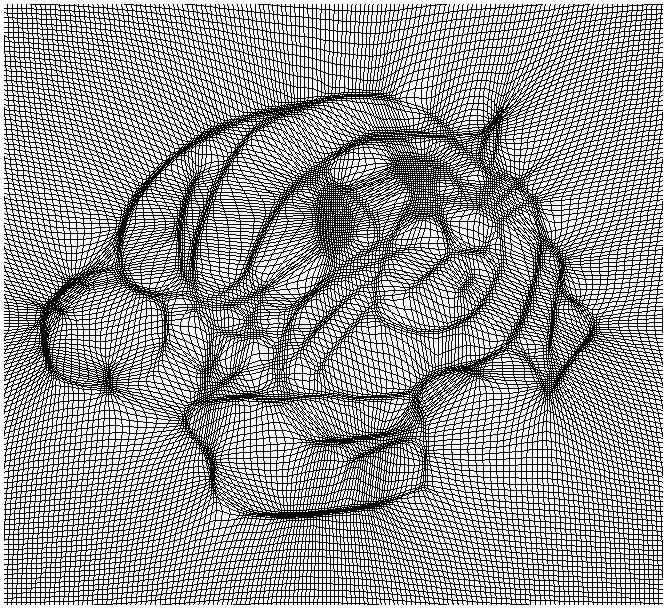
\includegraphics[width=0.45\linewidth]{cat_mesh1}}
}
\caption{Стационарная адаптация сетки путем перераспеделения узлов у произвольно заданной функции сеточной плотности. (a) заданная функция сеточной плотности $\rho$, (б) результат адаптации к заданной функции $\rho$.}
\label{fig:matroskin}
\end{figure}